\chapter[Declarative Optimization]{Declarative Optimization}
\label{ch:evita}

Declarative Networking and related topics have the potential to expand the lessons and 
impact of database technologies into new domains, while reviving interest in classical 
database topics like recursive query processing that had received minimal attention in 
recent years.  Yet our own systems were entirely implemented in imperative programming
languages: the initial version of the P2 runtime was implemented in C++~\cite{p2:sosp}, 
and the DSN declarative sensor network system began with an embedded dialect 
of C~\cite{chu-sensys07}. We asked ourselves whether Codd's vision applies to our own 
efforts: can declarative programming improve the implementation of declarative systems?

In this chapter, we put declarative systems ``in the mirror,''
investigating a declarative implementation of a key aspect of a
declarative system.  Specifically, we reimplemented the query
optimizer of P2 as a {\em metacompiler}: a compiler (optimizer) for the
P2 language, \OVERLOG, that is itself written in \OVERLOG.  We named the
resulting implementation ``Evita Raced.''\footnote{``Evita Raced'' is
almost ``Declarative'' in the mirror, but as with the \OVERLOG language
itself, it makes some compromises on complete declarativity.}  Using
Evita Raced, we extended P2 with a number of important query
optimization techniques it formerly lacked, and found that our
declarative infrastructure made this quite elegant and compact. For
example, our implementation of the traditional System R dynamic
programming algorithm comprises only 38 \OVERLOG rules (225 lines of
code); our implementation of the Magic Sets Rewriting optimization for
recursive queries is not only compact (68 rules, 264 lines), but also
nearly a direct translation of the description from Ullman's course
notes on the subject~\cite{ullmanNotes}.   

The elegance of our approach was derived in part from the fact that query optimization 
techniques -- like many search algorithms -- are at heart recursive algorithms, and
benefit from a declarative approach in much the same way as networking
protocols.  Even non-recursive optimization logic -- such as parts of
Ullman's magic-sets algorithm -- was simple enough to express in a
declarative fashion that abstracts away mechanistic details such as the
scheduling of data-parallel steps (e.g., scanning all rules in a program
in parallel versus sequentially).

Our contributions here are three-fold.  First, we presented a declarative architecture for query optimization 
that is based on metacompilation, reusing the query executor in a stylized fashion to serve as the engine beneath 
the optimization process.  This resulted in an {\em economy of mechanism}~\cite{Saltzer75theprotection}
not afforded by earlier extensible optimizers. Second, we showed that a variety of traditional and novel 
query optimizations are easy to express in a recursive, declarative language. Finally, 
we evaluated the simplicity and applicability of our design via a full-fledged implementation 
of an \OVERLOG query optimizer for the P2 Declarative Networking engine, which also 
cross-compiles code that runs on the DSN wireless sensor network platform~\cite{chu-sensys07}.  
Based on our experience, we believe that declarative metacompilation is a clean,
architecturally parsimonious way to build the next generation of extensible query optimizers
for a wide variety of emerging application domains, where the relevant optimizations remain
unclear.

The remainder of this chapter is organized as follows. In Section~\ref{ch:evita:sec:compile}, we describe
the steps to compile an \OVERLOG program into a relational representation. By compiling code into 
data, we are able to express optimizations and rewrites as queries. Section~\ref{ch:evita:sec:stages} 
packages these meta-queries into compilation stages that are dynamically installed into the compiler 
at runtime, using the same compilation path taken by any \OVERLOG program. In this dissertation, we describe 
three compilation stages that contain declarative specification of the System R dynamic program (Section~\ref{ch:evita:sec:systemr}), 
the Magic-sets rewrite (Section~\ref{ch:evita:sec:magic}), and the localization rewrite (Section~\ref{ch:evita:sec:localization})
for handling distributed joins in \OVERLOG~\cite{loo-sigmod06}. Section~\ref{ch:evita:sec:related} describes some
of the related work and Section~\ref{ch:evita:sec:summary} reflects on some lessons learned.

\section{Declarative Compilation}
\label{ch:evita:sec:compile}

Evita Raced is a compiler (i.e., query optimizer) for the \OVERLOG
declarative language that supports a runtime-extensible set of program
rewrites and optimizations, which are themselves expressed in \OVERLOG.
This metacompilation approach is achieved by implementing optimization
via dataflow programs  (query plans) running over a set of tables.  Two
main challenges must be addressed to make this work.  First, all
compiler state -- including the internal representation of both
declarative \OVERLOG programs and imperative dataflow programs -- needs
to be captured in a relational representation so that it can be
referenced and manipulated from \OVERLOG.  Second, the (extensible) set
of tasks involved in optimization must itself be coordinated via a
single dataflow program that can be executed by the P2 runtime engine.
In this section we describe the implementation of the Evita Raced
framework, including the schema of the compiler state, the basic
structure of the Evita Raced dataflow graph, and the basic dataflow
fragments needed to bootstrap the optimizer.

\begin{figure*}
\ssp
\begin{center}
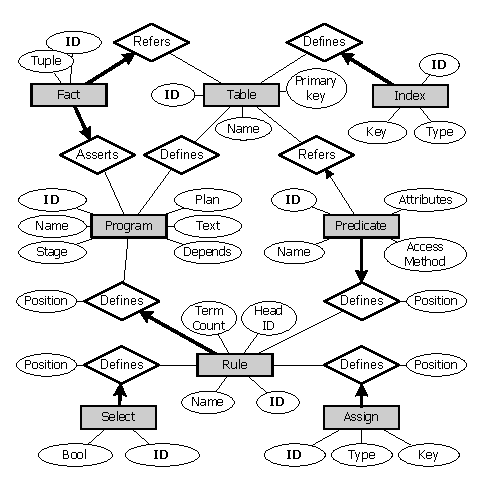
\includegraphics{figures/ERDiagram}
\caption{{ER Diagram of a query plan in P2. The primary key columns shown in bold.}}
\label{ch:evita:fig:p2er}
\end{center}
\end{figure*}
\subsection{Table-izing Optimizer State}
A typical query optimizer maintains a number of data structures to describe the contents 
of a query, and to represent ongoing properties of a query planner including fragments of 
query plans.  Our first task in designing Evita Raced was to capture this information in a 
relational schema.

Figure~\ref{ch:evita:fig:p2er} shows an Entity-Relationship diagram we developed that captures the 
properties of an \OVERLOG program, and its associated P2 dataflow query plans. 
We derived the constraints in the diagram by reviewing the semantic analysis rules enforced 
in the original P2 compiler; we discuss a few of them here for illustration.
An \OVERLOG~{\em rule} must appear in exactly one {\em program}. A {\em select} term 
(e.g., \ol{f\_contains(X,P2) == false} in Figure~\ref{ch:p2:fig:overlogSP}) is a Boolean expression 
over attributes in the predicates of the rule, and must appear in exactly one {\em rule}.  
The diagram indicates that a {\em predicate} must also appear in a unique {\em rule}, and 
that it may possibly reference a single {\em table}. A predicate that references a table is called 
a {\em table predicate} (or a \emph{materialized predicate}), while one that does not is called 
an {\em event predicate}. An {\em index} is defined over exactly one {\em table}, and a {\em table} 
defines at least one index (namely the primary key index, which P2 always
constructs). Some relations may contain {\em facts} (input tuples) at startup, 
each of which must belong to a single program and must reference a single table.

\begin{table*}
\small{
\begin{tabular}{|l|l|l|} \hline
{\it Name}& {\it Description} & {\it Relevant attributes} \\ \hline\hline
table     & Table definitions & {\bf table\_id}, primary\_key\\ \hline
index     & Index definitions & {\bf index\_id}, {\bf table\_id}, keys, type \\ \hline
fact      & Fact definitions  & {\bf program\_id}, {\bf table\_id}, {\bf id}, tuple\\ \hline
program   & User program description     & {\bf program\_id}, name, stage, text, depends, plan \\ \hline
rule      & Rules appearing in a program   & {\bf program\_id}, {\bf rule\_id}, name,  term\_count, head\_id \\ \hline
predicate & Relational predicates  & {\bf id}, {\bf rule\_id}, table\_id, name, position, access\_method \\ \hline
select    & Selection predicates  & {\bf id}, {\bf rule\_id}, boolean, position \\  \hline
assign    & Variable substitution statements & {\bf id}, {\bf rule\_id}, variable, value, position \\ \hline 
\end{tabular}
}
\ssp
\caption{The Metacompiler Catalog: tables defining an \OVERLOG program and dataflow execution plan.
                The primary key columns shown in bold. }
\label{tbl:catalog}
\end{table*}

The conversion from ER diagram to relational format was straightforward. Table~\ref{tbl:catalog} lists the set of relations that capture the entities 
mentioned in the ER diagram; we refer to this as the {\em Metacompiler Catalog}. We modified P2 to create these tables
at system startup, and they are accessible to any \OVERLOG programs (e.g., optimizations) subsequently added to the system.
% In addition, there are compiler constraints
% that cannot be captured by key constraints alone. For instance, a rule must contain
% exactly one head and one event predicate. Such checks can be performed by integrity 
% constraints written into the compiler logic (possibly as \OVERLOG programs). 

\subsection{Metacompiler Architecture}
\label{ch:evita:sec:metaarch}
Optimization logic expressed in \OVERLOG is declarative, and Evita Raced realizes this logic by converting it to a dataflow program to be executed by the P2 dataflow subsystem.  In this section we describe how Evita Raced represents query optimization programs as dataflow, and also the way it orchestrates multiple different optimization programs through the P2 dataflow framework.

An optimizer built using Evita Raced is composed of an extensible number of {\em stages}, each of which performs some
compilation task on the input program. One way to write an Evita Raced stage is to construct a dataflow program of one or more P2 elements in C++, and compile the result into the P2 binary; this is how we implement certain base stages required for bootstrapping, as described in Section~\ref{ch:evita:sec:bootstrap}.  However, the power of Evita Raced comes from its support for stages written in \OVERLOG, which, in addition to being compactly expressed in a high-level language, can be loaded into a running P2 installation at any time. 
A stage programmer registers a new stage with Evita Raced by inserting a tuple into the {\em program} relation. 
This tuple contains a unique identifier ($program\_id$), a name
($name$),  a list of stage dependencies ($depends$), and the program
text ($text$). Because the \ol{program} relation is used to convey
partial compilation results from stage to stage as well, \ol{program}
tuples also contain attributes for the name of the compiler stage operating 
on the program ($stage$), and the final physical plan ($plan$), though
these attributes are empty when the programmer first creates the tuple. Section~\ref{ch:evita:sec:stageschedule} describes the
$depends$ attribute, and its use in the installation of new stages. The $plan$ attribute pertains to the
physical planner stage, which is described in Section~\ref{ch:evita:sec:planner}.
We also expose the dataflow registration facility of Evita Raced to programmers inserting arbitrary
\OVERLOG programs  (not compiler stages) into a P2 node; for these generic programs, the $depends$ attribute must be empty.  We next describe the 
interfaces to an Evita Raced compiler stage, after which we discuss the way that multiple such stages are coordinated.

\subsubsection{The Stage API}
At base, an Evita Raced stage can be thought of as a stream query that listens for a tuple to arrive on an event stream called \ol{<stage>::programEvent}, where \ol{<stage>} is the name of the stage. 
The \ol{<stage>::programEvent} table contains all the attributes mentioned in the \ol{program} table. When such a tuple arrives, the stage runs its dataflow over that event and the tables in the Metacompiler Catalog, typically modifying catalog tables in some way, until it inserts a new \ol{program} tuple, containing the name of the stage in
the $stage$ attribute, into the program table. This insertion indicates
the completion of the stage.

To represent this behavior in a stage written in \OVERLOG, a relatively
simple template can be followed.  An \OVERLOG stage must have at least
one rule body containing the \ol{<stage>::programEvent} predicate. This 
represents the ability of the stage to react to new programs arriving at
the system.  In addition, the stage must have
at least one rule that
inserts a \ol{program} tuple into the \ol{program} table to signal stage
completion.  \OVERLOG stages may be recursive programs, so they run
to fixpoint before completing.

\subsubsection{Stage Scheduling}
\label{ch:evita:sec:stageschedule}
In many cases, optimization stages need to be ordered in a particular way for compilation to succeed.  For example, 
a {\em Parser} stage must run before any other stages, in order to populate the Metacompiler Catalogs, and an 
{\em Installer} stage must follow all other stages, since by installing the dataflow program into the P2 runtime it 
terminates compilation. We will see other specific precedence constraints in Section~\ref{ch:evita:sec:stages}.  


A natural way to achieve such an ordering would be to ``wire up'' stages explicitly so that 
predecessor stages directly produce \ol{<stage>::programEvent} tuples for their successors, 
in an explicit chain of stages.  However, it is awkward to modify such an explicit dataflow configuration 
upon registration of new stages or precedence constraints. Instead, Evita Raced captures precedence 
constraints as {\em data} within a materialized
relation called \ol{StageLattice}, which represents an arbitrary partial
order (i.e., an acyclic binary relation) among stages; this partial
order is intended to be a lattice, with the {\em Parser} as the source,
and the dataflow {\em Installer} as the sink.  (We review built-in stages in Section~\ref{ch:evita:sec:bootstrap}.)
 
To achieve the dataflow connections among stages, the built-in {\em
  StageScheduler} component listens for
updates to the \ol{program} table, indicating the arrival of a new
\OVERLOG program or the completion of a compiler
stage for an on-going program compilation, as described in the previous section.  The {\em StageScheduler} is
responsible for shepherding compilation stage execution according to the
\ol{StageLattice}. Given a \ol{program} update, it checks the lattice to identify a next stage
that can be invoked, and generates the
\ol{<stage>::programEvent} tuple that will start that stage; the
contents of the tuple are the same as those of the updated
\ol{program} tuple.  

\begin{figure*}[htbp]
\begin{center}
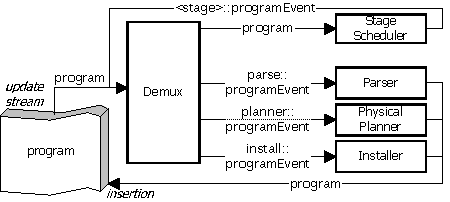
\includegraphics{figures/DefaultCompiler}
\ssp
\caption{The cyclic dataflow of Evita Raced, showing only the default compilation stages.}
\label{ch:evita:fig:basecompiler}
\end{center}
\end{figure*}

The StageScheduler and any compilation stages (whether built-in or
runtime-installed) are interconnected via the simple dataflow
illustrated in Figure~\ref{ch:evita:fig:basecompiler}. This is the same dataflow
that P2 constructs for all \OVERLOG programs. It consists of a C++ ``demultiplexer'' that
routes tuples from its input (on the left) to individual event handlers listening for
particular tuple names (the arrows leaving the Demux element in the
figure contain the name of the tuple for which the four components to the
right listen).  We did not changed P2's dataflow architecture~\cite{p2:sosp}, and its
details are not required for the rest of this chapter.  

Consider the simplicity of this approach as compared to the explicit
stage-wiring  sketched above. When a new compilation stage is installed
at runtime, the Installer (Section~\ref{ch:evita:sec:installer})
simply connects it to the {\em Demux} element, listening for
\ol{<stage>::programEvent} tuples, before updating the corresponding
tuple in the \ol{program} table. 
Then the StageScheduler who receives the updated \ol{program} tuple uses
the value of its $depends$ attribute  to insert appropriate 
\ol{StageLattice} tuples into the corresponding table of the
system catalog. Subsequent \ol{program} tuples being compiled will be directed to
the newly installed compiler stage by the StageScheduler as the updated
\ol{StageLattice} dictates.

To sum up, the life cycle of a program compilation starts when a user
submits a \ol{program} tuple to the system with a \ol{null} stage
attribute. The StageScheduler receives that \ol{program} tuple and
generates a
\ol{parse::programEvent} tuple (the Parser being the source stage in the
lattice), which is routed by the Demux element to
the Parser stage. When the Parser is done, it updates that \ol{program} tuple
in the corresponding table, changing the tuple's attribute to
``Parser.''  The StageScheduler receives the \ol{program} tuple, and routes a
\ol{planner::programEvent} to the Demux and eventually the Physical Planner, which goes round the loop again to the
Installer.  Finally, once the Installer is done and notifies the
StageScheduler via a \ol{program} tuple with the \ol{stage} attribute set to
``Installer,'' the StageScheduler concludes the compilation process.
If the \OVERLOG program being parsed is itself a new compilation stage, then after
installation, the scheduler updates the stage lattice.


\subsection{Compiler Bootstrapping}
\label{ch:evita:sec:bootstrap}
The previous architectural discussion neatly sidestepped a natural question: how is an Evita Raced compiler containing many \OVERLOG stages bootstrapped, so that it can compile its own \OVERLOG specification?
As in many metaprogramming settings, this is done by writing a small bootstrap  in a lower-level language. Evita Raced is initialized by a small C++ library that constructs the cyclic dataflow of Figure~\ref{ch:evita:fig:basecompiler}, including the three default stages shown, which are themselves written in C++. %The entire bootstrap, including the stages is {\bf XXX} lines of C++ (and a).  
Together, this code is sufficient
to compile simplified \OVERLOG (local rules only, no optimizations) into
operational P2 dataflows. We next describe each of these stages in a bit
more detail, since they form the foundation of the Evita Raced runtime.


% \jmh{This paragraph was saved from a conflict with Tyson's checkin.  Joe will merge it in Tuesday night.
% The {\em stage scheduler} is a dataflow element that is responsible for providing the inputs to a 
% stage and processing any outputs from a stage. The input to a stage module is a tuple containing the 
% identifier of the program that it is responsible for
% processing. When the stage completes its task is will insert a new program tuple into
% the \ol{program} table with an updated $state$ attribute value that indicates (to the scheduler) the completion 
% of the stage operation on the input program. The program insertion triggers a new
% \ol{programEvent} tuple that is again directed to the stage scheduler, and the process repeats with
% the next scheduled stage in the compilation order. Stage execution order is determined by
% a relation of stage dependencies. The stage scheduler schedules
% a stage based on the dependency graph relation installed by the bootstrap process and the current 
% value of the $state$ attribute in the program tuple. The process completes when the program $state$ 
% attribute reaches stage that no other stage depends on.
% }


% \subsubsection{Default Query Compilation}
% 
% Figure~\ref{ch:evita:fig:basecompiler} shows a dataflow perspective of our default
% metacompiler. A user submits a new program to the system by inserting a tuple into the \ol{program} table.
% The program tuple contains initial values for all the attributes in the program table (see Table~\ref{tbl:tables}). 
% A program table insertion triggers a \ol{programEvent} event tuple that contains the program 
% identifier attribute value.  The "Demux" dataflow element routes the \ol{programEvent} tuple to the
% stage scheduler element, which determines the order in which a stages execute on the input
% program. 
% \petros{The job of the scheduler is a bit nebulous. Is there something
% you can say here to make clear what that does?}
% 
% 
% The input to a stage module is a tuple containing the identifier of the program that it is responsible for
% processing. When the stage completes its task is will insert a new program tuple into
% the \ol{program} table with an updated $State$ attribute value that indicates (to the scheduler) the completion 
% of the stage operation on the input program. The program insertion triggers a new
% \ol{programEvent} tuple that is directed to the stage scheduler, and the process repeats with
% the next scheduled stage in the compilation order. Stage execution order is determined by
% a relation of stage dependencies. The stage scheduler schedules
% a stage based on the dependency graph and the current value of the $State$ attribute in the program tuple. 
% The process completes when the program $State$ attribute reaches stage that no further stage depend on.
% 
\subsubsection{Parser}

The Parser passes the program text it receives in the \ol{programEvent}
through a traditional lexer/parser library specified using
flex~\cite{flexUrl} and bison\cite{bisonUrl}; this library code returns
a standard {\em abstract syntax tree} representation of the text.
Assuming the Parser does not raise an exception due to a syntax error,
it walks the abstract syntax tree, generating Metacompiler Catalog
tuples for each of the semantic elements of the tree. In addition to
recognizing the different terms of each rule, the parser also annotates
each term with its position in the given program.  By convention, the
first term of a rule body is the event predicate of the rule, if one
exists.  By the same convention, the term in the last position for a
rule is the head predicate.



\subsubsection{Physical Planner}
\label{ch:evita:sec:planner}

The Physical Planner stage is responsible for doing a na\"{i}ve
translation of Metacompiler Catalog tuples (i.e., a parsed \OVERLOG program) into a dataflow program. It essentially takes each rule and deterministically translates it into a dataflow graph language, based on the positions of terms in the rule.

More specifically, for each rule the Planner considers each term
(predicate, selection or assignment) in order of position attribute.
The predicate representing the event stream is always planned first,
and registers a listener in the Demux element (recall
Figure~\ref{ch:evita:fig:basecompiler}).  The terms following the event stream
are translated, left-to-right, into a C++ dataflow in the same way that
the original P2 system did, so we do not address them further here.

We do mention three specific details. First, whereas the original P2
system translated a logical query plan directly to a software dataflow
structure in C++, we have chosen to create an intermediate, textual
representation of the dataflow. This representation is in a language
akin to the Click router's dataflow language, but we omit its details here. 

Second, unlike the original P2
system, we have introduced a number of access methods for in-memory
tables. Our \ol{predicate} relation contains the access method as one of
the attributes, and we have modified the P2 physical planner to choose
the appropriate dataflow element that implements the given access
method. 

%% Those are naturally introduced to the P2 physical planner
%% machinery and otherwise
%% creates
%% a listening port in the P2 {\em Demux} on the event stream name. The predicates mentioned in the rule that
%% do not represent the event stream represent lookup operations (joins) on the referenced base relation.
%% A join operator is planned for a predicate by taking the input stream and schema and joining 
%% it - using the $access\_method$ given by the \ol{predicate} tuple - with a base relation producing a new tuple 
%% stream with the join schema. 
%% A selection term plans a filter operator that applies the $boolean$ attribute value to the input 
%% stream and passes only tuples that satisfy this expression to the output stream. \jmh{Again the "plans an operators that does X" doesn't mean much to me.}An assignment term 
%% plans a assignment operator that uses the input stream to evaluate the $value$ attribute (in the \ol{Assign}
%% tuple) to an atomic value. If the input stream contains an attribute named by $variable$ 
%% (in the \ol{Assign} tuple) then the value of that attribute is substituted in the input
%% stream, otherwise a new attribute is added to the input schema with the given value 
%% in the output stream. After all rule body terms have been planned, the planner adds a projection operator
%% that projects the output tuple stream onto the head predicate.

% generates a physical plan for each rule in a program. The execution order of a physical plan in 
% P2 is a leaf-to-root path, with the leaf corresponding to the event predicate and the root being the head 
% predicate. All predicates that lie in between the leaf and the root path are joined against the respective 
% base relation according to the access method given by the predicate tuple. 
% \petros{I would go as far as saying that the physical plan you derive is
% expressed in an operator language reminiscent of the Click
% language. Since we concentrate on logical plan manipulations here we
% don't go into details. The important thing to point out is that whatever
% you do is not tied to a particular runtime; one could take this physical
% plan and install it on a different runtime that isn't our dataflow but
% something else.}

% The initial operator is always the event predicate and it determines when the rule should fire. 
% If the rule does not contain an event predicate then a delta rewrite must be preformed on the rule. 
% The delta rewrite converts the original rule into a set of new rules
% that trigger whenever a side affect\petros{``side affect'' should be
%   ``side effect'' everywhere.} 
% occurs on a table predicate mentioned in the original rule. The delta rewrite is presented 
% in~\cite{boonSigmod}, and we fully adopt this rewrite in our metacompiler. The position attribute 
% defined by each predicate tuple determines the position of the corresponding physical operator in 
% the physical plan. Select and assign operators are also planned at the position indicated by the 
% respective table tuple.

Third, as mentioned before, \OVERLOG rules may have no event predicate
(e.g., ``\ol{table1 :- table2, table3.}''). 
The physical planner converts such rules to (multiple) event rules via the {\em delta
rewrite} of Loo, et al.~\cite{loo-sigmod06}. (E.g., ``\ol{table1 :- delta\_table2,
table3.}'' and ``\ol{table1 :- table2,
delta\_table3.}''.) As in~\cite{loo-sigmod06} \ol{delta\_table} denotes a stream conveying
insertions, deletions, or timeout refreshes to tuples of the table
\ol{table}.


\subsubsection{Plan Installer}
\label{ch:evita:sec:installer}

Given the output of the Physical Planner in the dataflow specification
language, what remains is to parse the
textual representation of the dataflow,  construct the
corresponding C++ elements, and ``wire them up'' accordingly. We have
implemented this 
``physical plan compiler'' in C++, and housed it within the
Installer stage.  Once these elements and their connections are
instantiated, the Plan Installer stage stitches them into the P2
runtime's overall dataflow graph, as described in~\cite{p2:sosp}.
As noted in~\ref{ch:evita:sec:metaarch}, this infrastructure made it easy for us to extend P2 with the ability to modify its dataflow graph at runtime,
a feature not available in the released system. 
% Since our focus here
% is on plan optimization, we omit the engineering
% details of that contribution.
% 

\subsection{Discussion}
The metacompilation approach of Evita Raced led us to naturally design the system extensibility around issues of data storage and dataflow, rather than library loading and control flow modifications.  While any rule-based system is easier to extend than a procedural system, the internal implementation of Evita Raced is especially elegant, due to our thorough embrace of the native dataflow infrastructure, which we use both to execute optimization code, and orchestrate stages via precedence tables and the StageScheduler cycle.  The result of this design is that
even a major addition to the Evita Raced compiler entails very minimal
modification to the runtime state: only the addition of a pair of
dataflow edges to connect up the new stage, and the insertion of
precedence tuples in a single table.  Beyond the StageScheduler and the three bootstrap stages, no additional extensibility code was added to P2 to support Evita Raced.

Despite its simplicity, Evita Raced is flexible enough that we have used it to enhance P2 with support for new languages at both its input and output.  First, by extending the Parser element and registering some \OVERLOG rules, we have been able to get P2  to optimize and rewrite programs written in a new language, which extends \OVERLOG with the ability to attest to the provenance of data in a manner similar to that of~\cite{abadi-netdb07}.  Second, we have been able to use Evita Raced to cross-compile \OVERLOG programs into dataflow specifications that execute on the DSN platform, a declarative networking system that runs on wireless sensor nodes~\cite{chu-sensys07}.
%  In Section~\ref{ch:evita:sec:dsn} we present results from running Evita Raced plans in DSN on Berkeley Mote hardware.  


\section{Query Compilation Stages}
\label{ch:evita:sec:stages}

% \jmh{This paragraph is thoroughly redundant with hte previous section and can be chopped.  However, it'd be nice to have some kinda warmup text here.}
% A compilation stage written in the P2 query language is dynamically installed into the compiler 
% at runtime, using the same compilation path taken by any \OVERLOG program. The stage programmer 
% inserts a program tuple containing the text of an \OVERLOG program. The programmer also specifies, 
% in the {\em depends} attribute of the program tuple, a single stage that should execute immediately 
% before the installed stage.  After the insertion into the program table, the stage scheduler receives 
% the \ol{programEvent} tuple, which it uses to access the program tuple. The program is processed
% by the stages that appear in the current dependency graph relation. The stages treat the program 
% no differently than any other program. Once the program has been successfully installed, the stage 
% scheduler will then notice that the $depends$ attribute of the program tuple contains a 
% reference to a preexisting stage. 
% The dependency reference informs the stage scheduler that installed program represents a new stage, and 
% that it should update the dependency relation accordingly. After performing the update to the dependency
% relation, the new stage will be included in the compilation process of future input programs. 

Having described the Evita Raced infrastructure, we now turn to the issue of specifying query optimizations 
in \OVERLOG.  In this section we describe three of the compiler stages we have developed for Evita Raced. 
Section~\ref{ch:evita:sec:systemr} discusses a dynamic programming optimizer stage akin to that of
System R. Section~\ref{ch:evita:sec:magic} describes a stage that performs magic-sets rewrite on recursive 
\OVERLOG programs. Finally, Section~\ref{ch:evita:sec:localization} describes our reimplementation in Evita Raced 
of the localization rewrite from Loo et al.~\cite{loo-sigmod06}. 

\subsection{System R Optimization}
\label{ch:evita:sec:systemr}

The System R optimizer paper by Selinger, et al. is the canonical textbook framework for database query optimization~\cite{selinger}.  The paper laid out for
the first time the notion that query optimization can be decomposed
into two basic parts: query plan cost
estimation and plan enumeration.  While this algorithm is traditionally implemented inside
the heart of a database system via a traditional procedural
programming language, both of these tasks are
naturally specified in a declarative query language.  To perform cost
estimation, System~R requires data statistics like relation
cardinalities and index selectivities; \OVERLOG is a fitting language to
collect these statistics, especially in a distributed fashion over all
relation partitions. In our description we omit statistics gathering.

We focus instead on the basic dynamic programming algorithm for the
state-space enumeration at the heart of the System R optimizer.  This
algorithm enumerates query plans for increasingly-large subgoals of the
query optimizer.  It fills in a dynamic programming table keyed by the
plan identifier.  The dynamic programming task is
to fill in this table with the lowest-estimated-cost query plan among
all plans producing an {\em equivalent} output relation (i.e., plans
composed of the same terms).  
In the System R optimizer, the {\em principle of
optimality} is assumed to hold: the lowest-cost solution to some
plan will be built from the optimal solutions to subplans.  Thus dynamic
programming can proceed in ``bottom-up'' fashion.  Each rule's event
predicate is the ``outermost,'' streaming relation in a query plan for the rule.  For a given rule,
the optimizer generates plans of size $k$ terms by appending a single
(thus unused)
term from the rule body to the optimal plan of
size $k-1$ terms.

% An
% aggregation query chooses optimal plans from the set of equivalent plans.
We first describe the rules for plan generation and conclude with the
rules for optimal plan selection.

\subsubsection{Plan Generation}
\label{ch:evita:sec:plangen}

\begin{figure*}
\ssp
\centering
\begin{boxedminipage}{\linewidth}
pg1 {\bf plan}(@A, Pid, Rid, PlanID, SubPlanID, Type, TypeID, \\
\datalogspace \xspace \xspace Plan, Schema, Card, Cost, Pos, AM, Sort, TermC) :- \\
\datalogspace {\bf systemr::programEvent}(@A, Pid, \_, \_, \_, \_, \_, \_),\\
\datalogspace {\bf rule}(@A, Rid, Pid, \_, \_, \_, \_, TermC),\\
\datalogspace {\bf predicate}(@A, PredID, Rid, \_, \_, \_, \_, Schema, Pos, \_, \_),\\
\datalogspace Pos == $1$,\\
\datalogspace PlanID := {\em f\_idgen()}, SubPlanID := $null$,\\
\datalogspace Type := "Predicate", TypeID := PredID,\\
\datalogspace Plan := {\em f\_cons}(PredID, $null$),\\
\datalogspace Card := $1$, Cost := $1$,\\
\datalogspace AM := "STREAM", Sort := $null$.
\end{boxedminipage}
\caption{\label{ch:evita:fig:planseed}Plan seed rule.}
\end{figure*}

Figure~\ref{ch:evita:fig:planseed} shows the optimizer rule  that creates
the initial plan for each rule from the event predicate. The \ol{plan} tuple
contains a query plan for a given rule, and the plan's \ol{size} reflects the number of
term identifiers in the $Plan$ attribute (i.e., the number of leaves in the plan tree). The optimizer listens on the \ol{programEvent} event stream in
rule \ol{pg1}, which will start the optimization process.  
The \ol{programEvent} tuple is subsequently joined with the \ol{rule} table along the 
$Pid$ (program identifier) attribute to obtain the set of rules defined in the input program. 
The resulting set of rule tuples are each joined with the \ol{predicate} table along the 
$Rid$ (rule identifier) attribute. The result of this join produces a tuple for each predicate term 
defined by a given rule. The predicate term assigned to position~$1$ ($Pos == 1$) is
by convention the event predicate term.  For each 
event \ol{predicate} tuple in each rule of the input program, rule \ol{pg1} adds a new 
plan to the \ol{plan} table. The $Plan$ attribute represents the initial plan list,
starting with the term identifier ($PredID$) that identifies streaming predicates.
Plan generation proceeds by appending term identifiers to this list when
constructing new plans from optimal subplans.

The optimizer defines a set of plan generation rules that extend the
best plan found with $k$ terms with a new thus far unused term from the
rule body. Each such rule joins the \ol{bestPlanUpdate} event predicate
(generated when a new $k$-term plan is found) with unused terms in the
rule. If the new term considered is a predicate, then the new plan
must define an access method
that identifies the physical join operator, which
takes the optimal subplan and ``joins it'' with the predicate table. The access methods we presently 
support are scanned and index-nested-loop-join, as well as merge-join. 
The rules for plan generation from rule predicates are defined around the supported access methods. 
Due to space constraints, we only show the rules that generate plans for nested-loop-join 
and index nested-loop-join access methods.\footnote{A complete description of our rules 
in an extended technical report is available to the conference chair
during double blind reviewing.}

\begin{figure*}
\ssp
\centering
\begin{boxedminipage}{\linewidth}
pg2 {\bf plan}(@A, Pid, Rid, {\em f\_idgen()}, PlanID, "Predicate", PredID, \\
\datalogspace \xspace Plan, Schema, Card, Cost, OuterPos+$1$, AM, $null$, TermC) :-\\
\datalogspace {\bf bestPlanUpdate}(@A, Pid, Rid, PlanID),\\
\datalogspace {\bf plan}(@A, Pid, Rid, PlanID, \_, \_, \_, OuterPlan, \\
\datalogspace \datalogspace OuterSchema, OuterCard, OuterCost, OuterPos, \_, \_),  \\   
\datalogspace {\bf predicate}(@A, PredID, Rid, \_, \_, Tid, \_, PredSchema, PredPos, \_, \_),\\
\datalogspace $PredPos < TermC$,\\
\datalogspace {\bf table}(@A, Tid, \_, \_, \_, \_, TCard, \_),\\
\datalogspace {\em f\_contains}(PredID, OuterPlan) == $false$,\\
\datalogspace Card := OuterCard * TCard / $10$,\\
\datalogspace Cost := OuterCost + (OuterCard * TCard),\\
\datalogspace AM := {\em f\_cons}("SCAN", $null$), \\
\datalogspace Plan := {\em f\_cons}(PredID, OuterPlan), \\
\datalogspace Schema := {\em f\_merge}(OuterSchema, PredSchema).\\
\\
pgn {\bf planUpdate}(@A, Pid, Rid, PlanID, SubPlanID, Sort) :- \\
\datalogspace {\bf plan}(@A, Pid, Rid, PlanID, SubPlanID, \_, \_, \_, \_, \_, \_, \_, \_, Sort, \_).
\end{boxedminipage}
\caption{\label{ch:evita:fig:plangen1}Scan-join access method.}
\end{figure*}

A nested-loop-join plan access method is generated for any table predicate appearing
in the rule body. Rule \ol{pg2} in Figure~\ref{ch:evita:fig:plangen1} generates a
(scanned) nested-loop-join 
plan on all rule body table predicates not mentioned in the $OuterPlan$ attribute of the \ol{plan}
predicate representing the subplan. The \ol{plan} tuple representing the subplan is joined with 
the \ol{predicate} (all predicate terms in the rule body) table followed by another join with 
the \ol{table} (all tables in the system) table. The result of these join operations produce all 
term predicates mentioned in the rule that have a matching table identifier definition. 
The selection predicate $PredPos < TermC$ ensures that we do not
consider the rule head predicate (last in the rule's terms by
convention). The function $f\_contains$ tests for containment of the predicate in the subplan (outer plan). 
Any tuples that meet the constraints imposed by this rule generate a new \ol{plan} 
tuple with the ``SCAN'' access method (since the predicate table will be scanned for each outer tuple). 
Each new plan tuple is given a new $Plan$ attribute that appends the $PredID$ to the $OuterPlan$ 
subplan attribute. 
The cardinality ($Card$) and cost ($Cost$) estimates are given values based on some costing 
measure, which in this case makes use of best plan cardinality and cost estimates, and the predicate 
table cardinality.

\begin{figure*}
\ssp
\centering
\begin{boxedminipage}{\linewidth}
pg3 {\bf plan}(@A, ...) :-\\
\datalogspace ...\\
\datalogspace {\bf table}(@A, Tid, Tablename, \_, \_, \_, TCard, \_),\\
\datalogspace {\bf index}(@A, Iid, Tablename, Key, Type, Selectivity),\\
\datalogspace {\em f\_contains}(PredID, OuterPlan) == $false$,\\
\datalogspace {\em f\_indexMatch}(OuterSchema, PredSchema, Key),\\
\datalogspace Card   := OuterCard * (Selectivity * TCard),\\
\datalogspace Cost   := OuterCost + Card,\\
\datalogspace AM := {\em f\_cons}(Type, Iid),\\
\datalogspace ...
\end{boxedminipage}
\caption{\label{ch:evita:fig:plangen2}Index-join access method (diff from Figure~\ref{ch:evita:fig:plangen1}).}
\end{figure*}

An index-nested-loop-join plan is generated by rule \ol{pg3} in Figure~\ref{ch:evita:fig:plangen2}. The main
difference between this rule and rule \ol{pg2} is the additional \ol{index} predicate, which
adds index definitions to the resulting table predicate tuples. The function {\em f\_indexMatch}
tests if the index can be used to perform the join using attributes from the best plan schema ($OuterSchema$)
and attributes from the predicate table ($PredSchema$). Any tuple results from this plan are assigned 
cardinality and cost estimates based on some cost function, which uses the additional index selectivity
information given by the $Selectivity$ \ol{index} predicate attribute.
We also support range predicates in our index-nested-loop-joins but do
not show the 3 relevant rules here.

A merge-join performs a join of a plan with a table predicate mentioned in the rule body along
some sorting attribute. The tuple set from the outer plan and the predicate table must
be ordered by the sorting attribute. The output of a merge-join operation preserves
the sorting attribute order. Therefore, the \ol{plan} predicate generated by the merge-join rule 
includes the sorting attribute in the value of the $Sort$ \ol{plan} predicate. We note that the $Sort$
attribute in the \ol{table} plan table identifies the sorting attribute of the table.
A $null$ valued $Sort$ attribute, in either the outer relation \ol{plan} predicate or the inner relation
\ol{table} predicate, means that the relation is unordered, and must be presorted prior to the merge-join operator.  
The cost of a merge-join operator depends on need to presort either relation. 

\subsubsection{Best plan selection}
\label{ch:evita:sec:bestplan}

\begin{figure*}
\ssp
\centering
\begin{boxedminipage}{\linewidth}
bp1 {\bf bestCostPlan}(@A, Pid, Rid, Plan1, Sort1, {\small \bf a\_min}<Cost>) :- \\
\datalogspace {\bf planUpdate}(@A, Pid, Rid, \_, Plan1, Sort1), \\
\datalogspace {\bf plan}(@A, Pid, Rid, \_, \_, \_, \_, Plan2, \_, \_, Cost, \_, \_, Sort2, \_), \\
\datalogspace {\em f\_setequals}(Plan1, Plan2), Sort1 == Sort2. \\
\\            
bp2 {\bf bestPlan}(@A, Pid, Rid, PlanID, Plan2, Cost) :- \\
\datalogspace {\bf bestCostPlan}(@A, Pid, Rid, Plan1, Sort1, Cost), \\
\datalogspace {\bf plan}(@A, Pid, Rid, PlanID, \_, \_, \_, Plan2, \_, \_, Cost, \_, \_, Sort2, \_), \\
\datalogspace {\em f\_setequals}(Plan1, Plan2), Sort1 == Sort2.\\
\\            
bp3 {\bf bestPlanUpdate}(@A, Pid, Rid, PlanID) :- \\
\datalogspace {\bf bestPlan}(@A, Pid, Rid, PlanID, \_, \_).
\end{boxedminipage}
\caption{\label{ch:evita:fig:bestplan}Best plan selection.}
\end{figure*}

Figure~\ref{ch:evita:fig:bestplan} shows two rules that select the best plan from a 
set of equivalent plans, in terms of the output result set and the ordering 
properties of the result set. The \ol{bestCostPlan} predicate picks the
plan with the minimum cost from the set of equivalent plans. This aggregation 
query groups along the program identifier, rule identifier, plan list, and sort
attribute. The function {\em f\_setequals} tests whether the set of term identifiers 
in the two argument plans are the same, regardless of the order. The inclusion of 
the sort attribute in the group condition enables the handling of what Selinger 
calls ``interesting orders''~\cite{selinger}, along with optimal subplans. A separate 
rule (not shown) retains only those plans with no ordering attributes ($Sort == null$) and 
with sort orders on attributes that participate in subsequent join and group by 
operations~\footnote{Overlog does not have a notion of an "order by" clause.}.
 
The aggregation rule \ol{bp1} triggers whenever a new plan is added to the \ol{plan} 
table (indicated by the \ol{planUpdate} event). Then, the \ol{bestCostPlan} predicate is used 
in rule \ol{bp2} to select the identifier of the best plan, which is inserted into the \ol{bestPlan} 
table. An update to the \ol{bestPlan} table triggers a new \ol{bestPlanUpdate} event that the 
plan generation rules, described in Section~\ref{ch:evita:sec:plangen}, use to build new candidate plans.


\subsubsection{Improving Selectivity Estimation}

For equality selection predications, our System R rules above support selectivity
estimates using a uniform distribution estimator given by the index. For more precise
estimates and to handle range predicates, we have defined declarative rules that produce
equiwidth histograms ({\em ew-histograms}); additional histogramming rules could be
added analogously. The creation of an ew-histogram is triggered by the installation of a
fact in a metadata table of the ew-histograms defined in the system. The metadata table 
contains the parameters of the histogram (i.e., the table name, the attribute position,
and the number of buckets). For example, the fact
\[
\ol{sys::ewhistogram::metadata}(@LOCALHOST, "pred", 3, 10).
\]
creates a ten bucket equi-width historgram on table \ol{pred} for the attribute in the
third position.

Each fact in the ew-histogram table triggers Evita Raced rules that themselves generate
new rules to create ew-histograms (determining bucket boundaries based on the bucket
count and the min and max values of the attribute), and to maintain bucket counts (performing
a count aggregation over the table attributes, grouped by the bucket boundaries). The compiler
stage that generates ew-histograms in this fashion consists of $23$ rules ($92$ lines). The 
histogram data is stored in relational format with each row corresponding to a single bucket.
To exploit these histograms, the cost and selectivity estimation in the \ol{plan} generation rules
in Figures~\ref{ch:evita:fig:plangen1} and~\ref{ch:evita:fig:plangen2} are modified to incorporate
a join with the histogram data relation, and based on the bucket boundaries obtain density 
estimations for a given selection predicate.

\subsection{Top-down Optimization}

The bottom-up, dynamic programming search strategy is a natural fit to a Datalog-based rule 
language. However, a top-down Cascades-style optimization strategy~\cite{cascades} is just
as natural and intuitive in Evita Raced. We briefly describe how we implemented the Cascades 
branch-and-bound algorithm in \OVERLOG using only $33$ rules ($204$ lines).

In the Cascades optimizer, plans are classified into {\em groups}. A group is an equivalence class
of plans that produce the same result. The optimizer generates groups in a top-down order and
within each group it searches for the cheapest plan, the {\em winner}. An upper bound is assigned
to each group. A plan (and all its subplans) is pruned if its cost exceeds the group upper bound.
The upper bound for a given group is initialized to the parent group upper bound (the root group 
upper bound is initialized to a cost of inifinity) and continuously updated as new winner plans
are discovered. The optimization terminates when a root plan group has fully explored or pruned
all possible plans. The winner plan in the root group is then chosen to be the best-cost plan.


\begin{figure*}
\ssp
\centering
\begin{boxedminipage}{\linewidth}
bp1 {\bf branch}(@A, Pid, Rid, f\_groupID(SubPreds), 0, SubPreds, Bound) :- \\
\datalogspace {\bf winner}(@A, Pid, Rid, GroupID, Cost), \\
\datalogspace {\bf branch}(@A, Pid, Rid, GroupID, Pos, Preds, Bound), \\
\datalogspace $Pos < f\_size(Preds)$, \\
\datalogspace Bound := Cost, \\
\datalogspace SubPreds := f\_removePredicate(Pos, Preds). \\
\end{boxedminipage}
\caption{\label{ch:evita:fig:bb} Evita Raced branch-and-bound generation in top-down optimization.}
\end{figure*}

Figure~\ref{ch:evita:fig:bb} gives the single recursive rule that drives the optimization by generating groups of plans in a top-down
order. A \ol{branch} tuple contains the information that identifies a given group. Specifically, it identifies
the group (\ol{GroupID}), a branch position (\ol{Pos}), the predicates (\ol{Preds}) in the plan, and a
bound (\ol{Bound}). A separate \ol{cost} relation maintains the cost of plans computed from the
physical properties assigned to it during the optimization. A plan of size $k$ is formed out of the current
best-cost plan of size $k - 1$ and the best-cost singe predicate plan. The base case of this
recursion costs single-table plans. A new plan will only be generated if its cost is less than the bound
values in the branch tuple containing the group to which the new plan belongs. 

Suppose the initial query is $A \Join B \Join C$. The optimizer first initalizes the \ol{winner} relation
with a tuple for each group (i.e., $ABC$, $AB$, $AC$, $BC$, $A$, $B$, $C$) each having a cost
of \ol{infinity}. A single rule seeds the recursive rule \ol{c1} in Figure~\ref{ch:evita:fig:bb} by initializing
the \ol{branch} relation with a tuple that defines the root group (i.e., $ABC$) and starts the optimization
at position $0$ with predicates ($A$, $B$, $C$) and a bound of \ol{infinity}. The recursion proceeds in a
top-down fashion. In the first step a new \ol{branch} tuple is generated that removes the predicate in position $0$
generating the group $BC$. Another rule will generate a branch group $A$ at the same time. The recursion returns
when a winner for group $ABC$ has been discovered, which occurs when groups $A$ and $BC$ have been fully
explored and the \ol{next} branch position (e.g., $1$) is set for group $ABC$. A group has been fully explored when its 
branch position reaches the end. As new winners are discovered the \ol{Bound} variable is updated with the
winning cost before proceeding to the next predicate. 

\subsection{Magic-Sets Rewrite}
\label{ch:evita:sec:magic}

Datalog-oriented systems like P2 perform a bottom-up (\emph{forward chaining}) evaluation 
on each rule, starting with known facts (tuples), and recursively resolving body predicates to the 
head predicate. The advantage of this strategy is that the evaluation is data driven (from known facts 
to possible deductions) and will not enter infinite loops for some statically verifiable \emph{safe} programs. 
In contrast, top-down (\emph{backward chaining}) evaluation (e.g., in the Prolog language), 
starts with the query predicates as the top-level goals, and recursively identifies rules whose head predicates 
unify with needed goals, replacing them with the subgoal predicates in the rule body, until all subgoals are 
satisfied by known facts or rejected when no further recursion is possible. The advantage of a top-down evaluation 
strategy is that it avoids resolving goals that are not needed by the posed queries.

\begin{figure*}[!t]
\ssp
\centering
\begin{boxedminipage}{\linewidth}
{\bf link}("localhost:10000", "localhost:10001").\\
{\bf link}("localhost:10001", "localhost:10002").\\
...\\
\\
r1 {\bf path}(@X, Y, P, C) :- \\
\datalogspace {\bf link}(@X, Y, C), P := f\_cons(X, Y). \\
\\
r2 {\bf path}(@X, Y, P, C) :- \\
\datalogspace {\bf link}(@X, Z, C1), path(@Z, Y, P2, C2),\\
\datalogspace f\_contains(X, P2) == false, \\
\datalogspace P := f\_cons(X, P2), C := C1 + C2. \\
\\
Query: path(@LOCALHOST, "localhost:10000", P, C).
\end{boxedminipage}
\caption{\label{ch:evita:fig:querySP}Relevant rules copied from Figure~\ref{ch:p2:fig:overlogSP}.}
\end{figure*}

Consider again a snippet of the shortest path program in Figure~\ref{ch:evita:fig:querySP}. 
The query asks for the shortest path from all nodes to node ``localhost:10000''. A bottom-up evaluation
applies the \ol{link} tuples to rule \ol{r1}, creating the initial {\tt path} tuples. Rule \ol{r2} derives all \ol{path} tuples,
while any \ol{path} tuples matching ``localhost:10000'' on their second attribute are returned by the programmer's 
query.  

The bottom-up evaluation generates some \ol{path} tuples that do not have ``localhost:10000'' in 
the second attribute and therefore cannot satisfy the programmer's query.  In contrast, a top-down
evaluation begins by unifying the query predicate with the head predicate of rules \ol{r1} and
\ol{r2}. Therefore, the \ol{path} predicate unification binds the $@X$ attribute to the current node
identifier and the $Y$ attribute to ``localhost:10000'' in both rules, which is carried over to the predicates 
in the rule body. The binding of $@X$ and $Y$ attributes in rules \ol{r1} and \ol{r2} means that these
rules will only look for tuples of the form \ol{path}$(LOCALHOST,"localhost:10000",P,C)$ as well as 
tuples that can help form such \ol{path} tuples, but nothing else.

The magic-sets rewrite is an optimization that can reduce the amount of computation in 
recursive Datalog queries by deriving only those tuples that are relevant to query predicates 
posed by a program. It does this by adding extra selection predicates to the rules of a program 
to emulate the goal-oriented execution of top-down evaluation (this is sometimes called 
\emph{sideways information passing} or SIP). Conceptually, given a rule of the form
\[
H_p \ \text{\ol{:-}}\  G_1, G_2, ..., G_k
\]
where $H_p$ is the head predicate $p$ and $G_{1,...,k}$ are the goal
predicates in the order of appearance in the rule, a magic-sets
algorithm intersperses selection predicates $s_{1,...,k}$ to generate rule
\[
H_p \ \text{\ol{:-}}\  s_1, G_1, s_2, G_2, ..., s_{k}, G_k
\]
Facts for these selection predicates are generated according to bindings of
attributes, in the user's query or other rule predicates in the program, to
constant values. In Evita Raced we created a magic-sets rewrite stage written in
Overlog. The Overlog rules are based on the description of the magic-sets algorithm
given in Ullman's course notes~\cite{ullmanNotes}, which operates in three phases: program analysis,
program rewrite, and filter population. A very brief overview by example follows.

\subsubsection{Magic-sets by example}

\begin{figure*}[!t]
\begin{center}
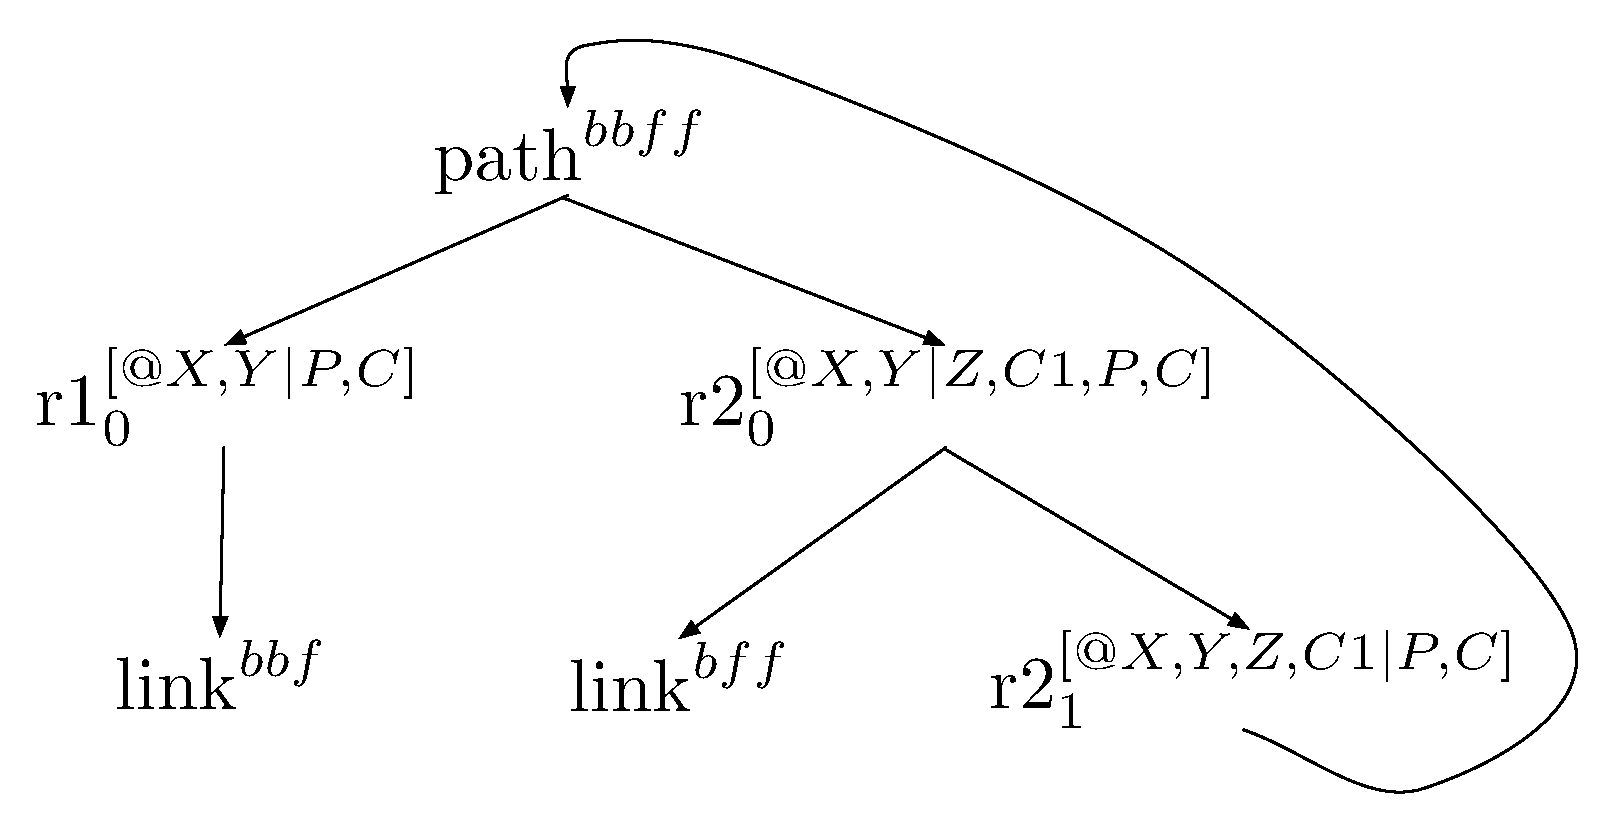
\includegraphics[scale=1.8]{figures/RuleGoalGraph}
\caption{Rule/Goal graph of the program in Figure~\ref{ch:evita:fig:querySP}.}
\label{ch:evita:fig:rggraph}
\end{center}
\end{figure*}

In the program analysis phase, the algorithm traverses every rule,
starting with those whose rule heads that match the query predicate, to build
a recursive tree structure called the {\em Rule/Goal} graph. This graph consists 
of \emph{rule} and \emph{goal} vertices.  A goal vertex consists of a predicate 
with an adornment indicating which of the attributes in the predicate are bound 
to a constant value and which are not (free).  A rule vertex represents the bound/free 
state of all seen variables within a rule body, up to a particular position in its left-to-right 
execution. A rule with $k$ body predicates will result in exactly $k$ rule vertices 
corresponding to its positions $[0,...,k-1]$.

Figure~\ref{ch:evita:fig:rggraph} illustrates the full {\em Rule/Goal} graph for our 
shortest path example.  To build this graph, the algorithm starts with a goal 
predicate (at first, this is the query predicate---\ol{path} in our example), and creates 
a goal vertex in the graph with the appropriate adornment ($\mathit{bbff}$ for
\ol{path} since the query binds its first two variables to constant values). For every
rule with that goal predicate as its head, the algorithm traverses the
rule body from left to right, creating a child rule vertex for every
$0$-th position variable binding.  For rule \ol{r2} in the example, the
rule vertex for position $0$ ($r_{2,0}$) has variable state $[X,Y|P,C]$,
which denotes that variables \ol{X,Y} are bound (to the same values as
those ``pushed down'' from the goal vertex) and \ol{P,C} are free.
Given a rule vertex for position $i$, two children are created: a goal
vertex for the next predicate after position $i$ and a rule vertex for
the next position in the rule (unless the body's end has been reached).
In the running example, the child goal vertex corresponds to the {\tt link} 
predicate that appears at position $0$, with adornment $\mathit{bff}$ 
since \ol{X} is already bound at this point in the evaluation, but \ol{Z, C1} are not.  
Similarly, the child rule vertex at position $1$ contains the variable signature 
$[X,Y,Z,C1|P,C]$ since \ol{link} added some bound variables.  The process 
continues until all rule and goal vertices have been constructed and connected; 
only a single goal vertex can exist with the same predicate and
adornment, as is the case for the \ol{path} vertex with adornment
$\mathit{bbff}$.  It is easy to see how the rest of the rule/goal graph is 
constructed. After all vertices have been generated given the chosen rules, 
any predicates with a unique adornment in the graph are added to the goals 
and the rules producing them are recursively traversed.


In the program rewrite phase, Ullman's algorithm traverses the rule/goal
graph generating magic predicates for each ``goal'' vertex that is
unique for its (IDB) predicate; in the example, there are multiple vertices
with different adornments for \ol{link}, but only one for \ol{path},
so only \ol{path} is chosen.  This magic predicate is inserted in
the $0$-th position of all rules with the corresponding goal predicate
as the rule head, with the bound variables of the signature as
attributes. In the example, the magic predicate for \ol{path} has the
form \ol{magic\_path(@X, Y)} since \ol{X, Y} are the bound 
variables in the signature of the ``goal'' vertex.  Also
\emph{supplementary} predicates are similarly created for all
encountered ``rule'' vertices during the graph traversal and inserted
within the corresponding original rule.  For example, {\tt sup\_r2\_1(@X,Y,Z,C1)} 
is created for ``rule'' vertex $r_{2,1}$ with the bound variables of
the adornments in the vertex, and placed in the original rule \ol{r2}
between the \ol{link} and \ol{path} predicates.


\begin{figure*}[!t]
\ssp
\begin{boxedminipage}{\linewidth}
{\bf link}("localhost:10000", "localhost:10001").\\
{\bf link}("localhost:10001", "localhost:10002").\\
...\\
{\bf magic\_path}(@LOCALHOST, "localhost:10000"). \\
\\
r1\_g3a {\bf path}(@X, Y, P, C) :- \\
\datalogspace {\bf magic\_path}(@X, Y), \\
\datalogspace {\bf link}(@X, Y, C), P := f\_cons(X, Y).\\
\\
r2\_g1a {\bf magic\_path}(@X, Y) :- \\
\datalogspace {\bf sup\_r2\_1}(@X, Y, Z, C1). \\
\\
r2\_g3a {\bf sup\_r2\_1}(@X, Y, Z, C1) :- \\
\datalogspace {\bf magic\_path}(@X, Y), \\
\datalogspace {\bf link}(@X, Z, C1). \\
\\
r2\_g3c {\bf path}(@X, Y, P, C) :- \\
\datalogspace {\bf sup\_r2\_1}(@X, Y, Z, C1), \\
\datalogspace {\bf path}(@Z, Y, P2, C2). \\
\datalogspace f\_contains(X, P2) == false, \\
\datalogspace P := f\_cons(X, P2), C := C1 + C2. \\
\\
Query: {\bf path}(@LOCALHOST, "localhost:10000", P, C).
\end{boxedminipage}
\caption{\label{ch:evita:fig:magicSP}A magic-sets rewrite of
      the rules in Figure~\ref{ch:evita:fig:querySP} (materialize statements not shown).}
\end{figure*}

Finally, in the filter population phase, the algorithm maintains the
magic predicate relation, which was placed within the rewritten program
in the previous phases.  Any a priori known bindings about the root goal vertex
(e.g., from the user's query) are placed in the magic relation. In the example, the 
fact ``\ol{magic\_path(LOCALHOST, "localhost:10000").}'' is put into the
database from the bindings in the \ol{path} query.  Also, any edges in
the rule/goal graph that start from a rule vertex and end at a goal vertex, with a
unique adornment (i.e., upward arrows in the recursive tree that constitutes the graph), are written as
rules that generate new magic tuples from new tuples of the rule
node's supplementary predicate. In the example, rule \ol{r2\_g1a}~\footnote{Rule names that
deal with magic and supplementary predicate maintenance were named according
to Ullman's rule groups. For instance, rules named \ol{r*\_g3[a-c]} follow rule group 3
and rule \ol{r2\_g1a} follows rule group 1.}  adds
more magic facts as more \ol{sup\_r2\_1} tuples are produced.

Our rewrite implementation of this algorithm first traverses every rule
from head predicate to body predicates from left to right, constructing
the rule/goal graph in the recursive manner of the program analysis, in
a single fixpoint.  Then the new program rules (and replacement of old
rules) for the program rewrite and filter population phases are
performed via a traversal of the newly constructed rule/goal graph in a
subsequent fixpoint. Finally, initial magic facts are created by direct
translation from the query.  Other details that we elide here involve detecting 
eligibility of a predicate for a magic-sets rewrite (whether or not it has a unique 
adornment in the rule/goal graph), state cleanup, etc. 

\begin{figure*}
\ssp
\begin{boxedminipage}{\linewidth}
{\bf materialize}(sup,infinity,infinity,keys(2,3,4)). \\
{\bf materialize}(adornment,infinity,infinity,keys(2,5,6)). \\
{\bf materialize}(idbPredicate,infinity,infinity,keys(2,3)). \\
\\
mg1 {\bf goalCount}(@A, Pid, PredName, a\_count$<*>$) :- \\
\datalogspace {\bf idbPredicate}(@A, Pid, PredName), \\
\datalogspace {\bf adornment}(@A, Pid, Rid, Pos, PredName, Sig). \\
\\
mg2 {\bf magicPred}(@A, Pid, GoalName, Sig) :- \\
\datalogspace {\bf goalCount}(@A, Pid, GoalName, Count), \\
\datalogspace {\bf adornment}(@A, Pid, \_, \_, GoalName, Sig). \\
\datalogspace Count == 1. \\
\\
mg3 {\bf sup}(@A, Pid, Rid, Pos, Name, Schema) :- \\
\datalogspace {\bf magicPred}(@A, Pid, Name, Sig), \\
\datalogspace {\bf rule}(@A, Rid, Pid, \_, HeadPid, \_, \_, \_), \\
\datalogspace {\bf predicate}(@A, HeadPid, Rid, \_, Name, \_, \_, Schema, \_, \_, \_), \\
\datalogspace Schema := {\em f\_project}(Sig, Schema), \\
\datalogspace Name := "magic\_" + Name, Pos := 0. \\
\\
mg4 {\bf supNext}(@A, Pid, Rid, Pos+1, Schema) :- \\
\datalogspace {\bf sup}(@A, Pid, Rid, Pos, Name, Schema). \\
\\
mg5 {\bf sup}(@A, Pid, Rid, Pos, Name, Schema) :- \\
\datalogspace {\bf supNext}(@A, Pid, Rid, Pos, PrevSupSchema),\\
\datalogspace {\bf rule}(@A, Rid, Pid, RuleName, \_, \_, \_, \_),\\
\datalogspace {\bf predicate}(@A, \_, Rid, \_, \_, \_, \_, Schema, Pos, \_, \_),\\
\datalogspace Name := "sup\_" + RuleName + "\_" + {\em f\_tostr}(Pos),\\
\datalogspace Schema := {\em f\_merge}(PrevSupSchema, PredSchema).\\
\\
mg6 {\bf adornment}(@A, Pid, Rid, Pos, PredName, Sig) :- \\
\datalogspace {\bf supNext}(@A, Pid, Rid, Pos, PrevSupSchema),\\
\datalogspace {\bf idbPredicate}(@A, Pid, PredName), \\
\datalogspace {\bf rule}(@A, Rid, Pid, \_, \_, \_, \_, \_),\\
\datalogspace {\bf predicate}(@A, \_, Rid, \_, PredName, \_, \_,Schema, Pos, \_, \_),\\ 
\datalogspace Sig := {\em f\_adornment}(PrevSupSchema, Schema).
\end{boxedminipage}
\caption{\label{ch:evita:fig:magicRules}Rule/Goal graph traversal rules.}
\end{figure*}

To give a flavor of the \OVERLOG implementation of magic-sets,
Figure~\ref{ch:evita:fig:magicRules} shows six rules that build the state
necessary in the magic-sets rewrite by traversing the rule/goal graph. 
The \ol{adornment} predicate contains the predicate name ($PredName$) and an
adornment string ($Sig$), which is initially populated (by a single rule, not shown) with
the query predicate adornments. Rule \ol{mg1} counts the number of
adornments for each {\em IDB} predicate. If this count is unique ($Count == 1$) in rule \ol{mg2},
then a \ol{magicPred} tuple is created. Rule \ol{mg3} triggers on a \ol{magicPred} tuple and, for each
rule whose head predicate is named by the \ol{magicPred} tuple, it generates a \ol{sup} predicate
with a $Schema$ attribute containing the bound variables that exist at the given rule position. 
Rule \ol{mg4} detects a new \ol{sup} predicate (like the one generated for the rule head) and triggers 
an event for the subsequent \ol{sup} predicate position in the given rule. The three way join in rule \ol{mg5} 
produces a tuple that contains the schema of the previous \ol{sup} predicate ($PrevSupSchema$) 
and the schema of the predicate ($Schema$) in the subsequent rule position, should one 
exist~\footnote{Two rules (not shown) move the \ol{supNext} position forward if the given rule position does 
not identify a predicate.}. The head \ol{sup} predicate schema in rule \ol{mg5} contains all the variables from the 
previous \ol{sup} predicate and the schema of the current predicate, since this schema represents the bound variables
that will exist in the subsequent rule position. Rule \ol{mg6} creates an \ol{adornment} out of the predicate 
in the given rule position, if that predicate is part of the {\em IDB}. The {\em f\_adornment} 
function creates a new signature from the bound variables in the $PrevSupSchema$ attribute, 
and the variables in the predicate $Schema$ attribute. At the end of the rule/goal graph traversal, 
those predicates that define a unique adornment become magic predicates, and the rules that mention 
these magic predicates are rewritten using the information contained in the \ol{sup} table.

\subsubsection{Magic-sets in the Network}

With the details of the magic-sets algorithm behind us, what is
intuitively happening to the shortest-path snippet in
Figure~\ref{ch:evita:fig:magicSP} is that variable bindings in the query are
recursively translated into filtering magic and supplementary
predicates. Since the query is only looking for paths to
destination ``localhost:10000'', at first the magic fact restricts single-hop
paths created from links in rule \ol{r1}) to only those with that same 
destination (in the rewritten rule \ol{r1\_g3a}). Similarly, in what used to 
be rule \ol{r2}, {\tt link} tuples are filtered according to the magic predicate (in rule
\ol{r2\_g3a}), before being joined with existing \ol{path} tuples to
complete the old rule \ol{r2}. The reason rule \ol{r2} was split into
the two rules \ol{r2\_g3a} and \ol{r2\_g3c} is because the
supplementary result \ol{sup\_r2\_1} is useful towards adding extra bindings as
magic tuples (in rule \ol{r2\_g1a}); this is because any variable
binding that survives filtering right before the \ol{path}
predicate in the body of the old rule \ol{r2} is also an interesting
binding for existing or future \ol{path} tuples. If the original
program had not been recursive, then such recursive definitions of magic
facts would not appear in the rewritten program.

\begin{figure*}
\centering

\includegraphics[scale=1.2]{figures/Topology}
\caption{Experimental topology.}
\label{ch:evita:fig:topo}
\end{figure*}

To understand the effects of this rewrite, we describe two experimental
runs of our program, before and after the magic-sets rewrite (both
programs were also subjected to the localization rewrite from
Section~\ref{ch:evita:sec:localization} since they are distributed).  The two
programs are executed in the simple link topology of
Figure~\ref{ch:evita:fig:topo}. Nodes are started up one at a time in order of
identifier, and the preloaded database (EDB) consists of the links pictured. For each experiment we measure the number of
tuples sent and received by each node, as well as any \ol{path}
tuples constructed. The latter measure is meant to convey ``work''
performed by the distributed program even in local computation that does
not appear on the network (e.g., local tuple computations, storage, and
other dependent actions on those tuples).

\begin{figure*}
\centering
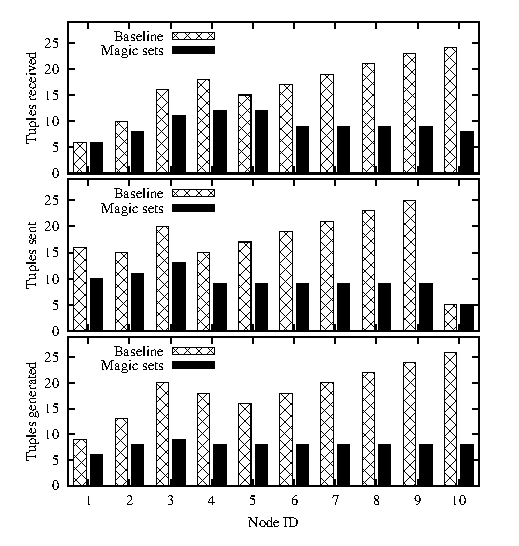
\includegraphics{figures/magicNumbers}
\ssp
\caption{For each node (node ID on $x$ axis), number of tuples received
  (top), sent (middle), and locally generated (bottom) on the $y$ axis.}
\label{ch:evita:fig:magicresults}
\end{figure*}

Figure~\ref{ch:evita:fig:magicresults}(a) shows the number of tuples that each node receives from
the network. The magic-sets rewritten program causes no more tuples to
be received than the original, and for most nodes significantly fewer
when moving to nodes farther away from the clique. That is because many
paths that are generated in the original program with destinations
within the clique other than node $1$ are pruned early on and never
transmitted all the way to the far end.    Similarly,
Figure~\ref{ch:evita:fig:magicresults}(b) shows the number of tuples each node transmits.
Again, the magic-rewritten program does a lot better.  The two programs
have similar tuple transmit/receive overheads for nodes represents the number of tuples a node sends out
over the network. The inclusion of the magic-sets rewrite reduces the number of sends
in all but one case (node $10$). The node with identifier $10$ is the only node with 
no incoming links and 
is therefore never burdened with network traffic other than its
own; as a result, though its received tuple overhead benefits from magic
sets, it transmitted tuple overhead is unaffected, since it already
sends out no extraneous paths other than its sole path towards node $1$.
Finally, tuple storage is impacted beneficially by magic sets everywhere
(Figure~\ref{ch:evita:fig:magicresults}(c)), since
both \ol{path} tuples received from the network, but also those
generated locally for local consumption are pruned away by the rewrite.



\subsection{Localization}
\label{ch:evita:sec:localization}

Finally, we briefly describe the localization compiler stage, which turns
a rule with  multiple
location specifiers in its body to many rules, each of which has a
single location specifier in its body; this essentially turns a
distributed join into a set of local joins with partial result
transmissions among the rules involved~\cite{loo-sigmod06}. This rewrite
is part of the P2
system, but implemented in C++ and woven into the monolithic compiler.

In Evita Raced, localization stage traverses distributed rules in
left-to-right order starting with first body predicates (rules with
local-only body predicates are selected out early in the stage). 
The location attribute of the current predicate in this traversal is noted at each iteration.
A {\em breakpoint} is generated if the traversal reaches a predicate with location attribute 
that differs from the previous. The breakpoint triggers a {\em split} rule at the given 
position, which creates a new {\em glue} predicate $IR_p$, and two new rules defined as follows.
\begin{CompactEnumerate}
\item $IR_p$ :- (predicates to the left, excluding the breakpoint).
\item (original rule head predicate) :- $IR_p$, (predicates to the right, including the breakpoint). 
\end{CompactEnumerate}
The location attribute in the $IR_p$ predicate is taken from the predicate at the breakpoint position.
The other attributes in the $IR_p$ predicate are taken from the predicates to the left of (and not 
including) the breakpoint, which represents the schema of the intermediate result prior to the
breakpoint position predicate. The algorithm then removes the original rule, and moves recursively on
the second rule, which is considered the original rule in the above discussion. 
The recursion terminates at the rightmost predicate position. 

The localization stage is not an optimization per se, but rather a  program rewrite necessary to make distributed rules executable. 
% Any program that contains distributed rules must go through this compilation stage. 
The \OVERLOG program for localization consists of only 28 rules. The original P2
code that performed this task in P2 consisted of approximately 400 lines of
% carefully crafted 
C++.  


\section{Related Work}
\label{ch:evita:sec:related}

The pioneering work on extensible query optimizer architectures was done in the EXODUS~\cite{exodus} and Starburst~\cite{lohman,phh92} systems, which provided custom rule languages for specifying plan transformations.  The EXODUS optimizer generator used a forward-chaining rule language to iteratively transform existing query plans into new ones. Follow-on work (Volcano~\cite{volcano} and Cascades~\cite{cascades}) exposed more interfaces to make the search in this space of transformations more efficient.  Starburst had two rule-based optimization stages.  The SQL Query Rewrite stage provided a production rule execution engine, for ``rules'' that were written imperatively in C; it included a precedence ordering facility over those rules.  The cost-based optimizer in Starburst was more declarative, taking a grammar-based approach to specifying legal plans and subplans.

While all of this work was rule-based and extensible, most of it only exposed individual plan transformations to extensibility; the actual search algorithms or transformation orderings of EXODUS, Volcano, Cascades, and the Starburst cost-based optimizer were fixed in procedural code.  By contrast, Evita Raced does not embed a search algorithm, instead leaving that open to specification as needed.  The dynamic programming search we implemented is a natural fit to a Datalog-based rule language, and it is an interesting future work challenge to consider whether the Cascades-style ``top-down'' optimization is easy to achieve in \OVERLOG; the fact that magic-sets rewriting blurs the difference between top-down and bottom-up logic evaluation may be germane here~\cite{topdownbottomup}.

Another interesting extensible query optimizer is Opt++~\cite{kabradewitt}, which exploits the object-oriented features of C++ to make an optimizer framework that was easy to customize in a number of ways.  A specific goal of Opt++ was to make the search strategy extensible, enabling not only top-down vs. bottom-up state-space enumeration, but also randomized search algorithms.  Evita Raced embraces these additional dimensions of extensibility introduced by Opt++, but provides them in a higher-level declarative programming framework.

The cyclic dataflow used for stage scheduling in Evita Races resembles the continuous query engine of TelegraphCQ, with our StageScheduler and Demux elements working together to behave somewhat like the TelegraphCQ {\em eddy} operator~\cite{tcq-cidr}.  This connection occurred to us long after we developed our design, but in retrospect the analogy is quite natural: Evita Raced stages are akin to TelegraphCQ's ``installed'' continuous queries, and P2's \OVERLOG queries are akin to data streaming into TelegraphCQ.

Our description of \OVERLOG was based on our understanding of the current state of the P2 codebase.  Loo et al.~\cite{loo-sigmod06} describe a language for P2 they call Network Datalog (NDLog), that is roughly a simple sub-language of the current state of \OVERLOG.  NDLog is a subset of Datalog with aggregation, and hence does not provide delete rules or updates.  Unlike \OVERLOG, NDLog offers well-defined global program semantics across the network, but it does so by not offering delete or update rules, which are used in many \OVERLOG programs.


\section{Discussion}
\label{ch:evita:sec:discussion}

When we started this work, the vision of declaratively specified query optimization was appealing 
thanks to its elegance and its promise of usability and maintainability.  Although we remain convinced 
on this front, our optimism has been tempered by the pragmatics of developing software within a
continuously changing system prototype. Here we reflect on some of the (hard) lessons we learned 
while conducting this research.

P2's notion of consecutive Datalog-style fixpoints, especially in networked environments, still has 
many rough edges, both on the design and on the engineering front.  Because deep down P2's runtime 
is an event-driven execution engine, its basic unit of atomicity is akin to a single iteration 
through a recursive query evaluation strategy like semi-naive evaluation, generating a set of 
derived actions (tuples to be inserted, deleted, transmitted remotely, or evaluated locally for 
further deduction) from a single incoming event, and committing changes to the database atomically 
upon completion of such a step~\cite{LuThesis}. P2's Datalog-style fixpoints are implemented as 
sequences of such single-event iterations, in a manner that appears to have been an afterthought. 
As a result, the system's design shares both event-driven and logic-style flavors, with some 
remaining unresolved conflicts, and no explicit language constructs to bridge between the two.

One example is the notion of \ol{delete} rules, the semantics of which are unclear.  How is one to 
handle delete rules triggered by the \emph{deletion} of a base tuple?  The system certainly does 
not support -- semantically or operationally -- the ``undeleting'' of tuples that were
originally deleted due to a base fact that is no longer in the database.  Similarly, the semantics 
for multiple updates to the same tuple within the same fixpoint are undefined and a local tie
breaking rule is chosen to decide on a consistent ordering among same-fixpoint updates to the 
same relation. Compiler stages that do static analysis might catch such dangerous rules and alert the user.

Second, as in most prototypes, the programmer interface is not polished. Debugging is difficult, especially 
since the logic language makes it tough to understand which value corresponds to which formal
attribute in a long tuple of a dozen or more attributes.  Though concise, declaratively specified 
optimizations pack a punch in terms of density of concepts, which only becomes deadlier due to the (otherwise
desirable) arbitrary order of rule execution.  Certainly a better thought-out system to debug declarative 
programs -- optimizations, no less -- would have made the job easier.  To be fair, however, our
experience with building monolithic optimizers in production database management systems in the past 
was not a great deal rosier.  It is hard to debug code when the output's correctness (e.g., minimality of cost) 
is too expensive to verify.

Third, the evolution of the \OVERLOG language has a long way to go. The language still offers no modularity, 
making it tough to isolate and reuse logically distinct components. It does has a rudimentary concrete
type system, but has poor support for structured types like matrices and lists.  \OVERLOG still ``cuts corners'' 
on the proper set-orientation of Datalog; since program stratification is only preliminary in
the system prototype, dealing with streaming aggregates in the face of EDB updates required us to 
resort to imperative tricks like timers and polling to determine that aggregates were ready to be finalized.

Beyond particular characteristics of P2, one hard lesson we learned was that extensibility and ease of use at 
the top often comes at the expense of complexity below the extensibility layer.  The tabularization of
compiler state to enable declarative optimizations also meant that even imperative compiler stages such as our
bootstrap stages implemented in C++ had to use tables, foregoing their familiar interaction with C++ data 
structures.  Building glue libraries that ease this interaction may relieve this pain.

Nevertheless, despite these complaints, we were able to get all of our desired optimizations expressed 
in \OVERLOG in a highly compact way, as promised by the various earlier papers on P2.  By contrast, the 
initial version of P2 had no query optimizations of interest beyond localization.  As \OVERLOG and P2 mature, 
the use of a metacompilation approach should get even easier.  And based on our initial experience 
extending \OVERLOG with security properties in a manner similar to~\cite{abadi-netdb07}, we believe that 
our Evita Raced infrastructure could accelerate the ability of the P2 group to pursue modifications to 
\OVERLOG itself.

\section{Summary}
\label{ch:evita:sec:summary}

The Evita Raced metacompilation framework allows \OVERLOG compilation tasks to be written in \OVERLOG and
executed in the P2 runtime engine. It provides significant extensibility via a relatively clean declarative
language. Many of the tasks of query optimization -- dynamic programming, dependency-graph construction
and analysis, statistics gathering -- appear to be well served by a recursive query language. The notion of
metacompilation also leads to a very tight implementation with significant reuse of code needed for
runtime processing.

Even with the caveats expressed in Section~\ref{ch:evita:sec:discussion}, we are convinced that a declarative metacompiler
is much easier to program and extend than the monolithic query optimizers we have worked on previously.
We are now at a  point where we can add significant features (e.g., histograms, broadcast rewrites, 
stratification tests) in an hour or two, where they would otherwise have taken days or weeks of work
in a traditional implementation. 

One surprising lesson of our work was the breadth of utility afforded by the metacompilation framework. Although
motivated by performance optimizations, we have used Evita Raced for a number of unforeseen tasks. These
include: automatically expanding user programs with instrumentation and monitoring logic; generating pretty-printers
for intermediate program forms; language wrappers for secure networking functionality in the manner of
SecLog~\cite{abadi-netdb07}; stratification detectors and other static code analysis. None of these are performance optimizations
per se, but all fit well within an extensible, declarative program manipulation framework. More generally, we believe
that metacompilation is a good design philosophy not only for our work, but for the upcoming generation of
declarative engines being proposed in many fields. 

